\section{ShEx Based Syntax}
\labsec{ch04-shex-subset-analysis}

ShEx as itsleft it is not a syntax, it is a specification described in \sidecite{eric-rdf-validation-lang} 
and for that specification multiple syntaxes where proposed and implemented \sidecite{labra-validating-rdf}.
One of those syntaxes is the \texttt{Compact} syntax, which main goal is to be human frindly. It is also
the chossen one for IDE's and other tools that directly communicate with humans and therefore will be the
one that we will choose to start from.

As the title and the main goal of this project said this syntax needs to be a subset of ShEx, this is done
in order to allow \textbf{interoperability}, that is, every schema defined in this subset syntax needs to be
\textbf{fully compatible with other ShEx tools}.

In order to analyze all the features that our syntax will include we will perform some use cases and from
them we will extract the requirements that the syntax will need to implement.

\subsection{Syntax Use Cases}

\reffig{shex-lite-syntax-use-case} sows the high level view of the use cases that we expect ShEx-Lite syntax
to be use for. Those use cases include the \textbf{definition of prefixes}, the \textbf{definition of the base},
the \textbf{definition of the start shape expression} and the \textbf{definition of shape expressions}.

\begin{figure*}[h!]
	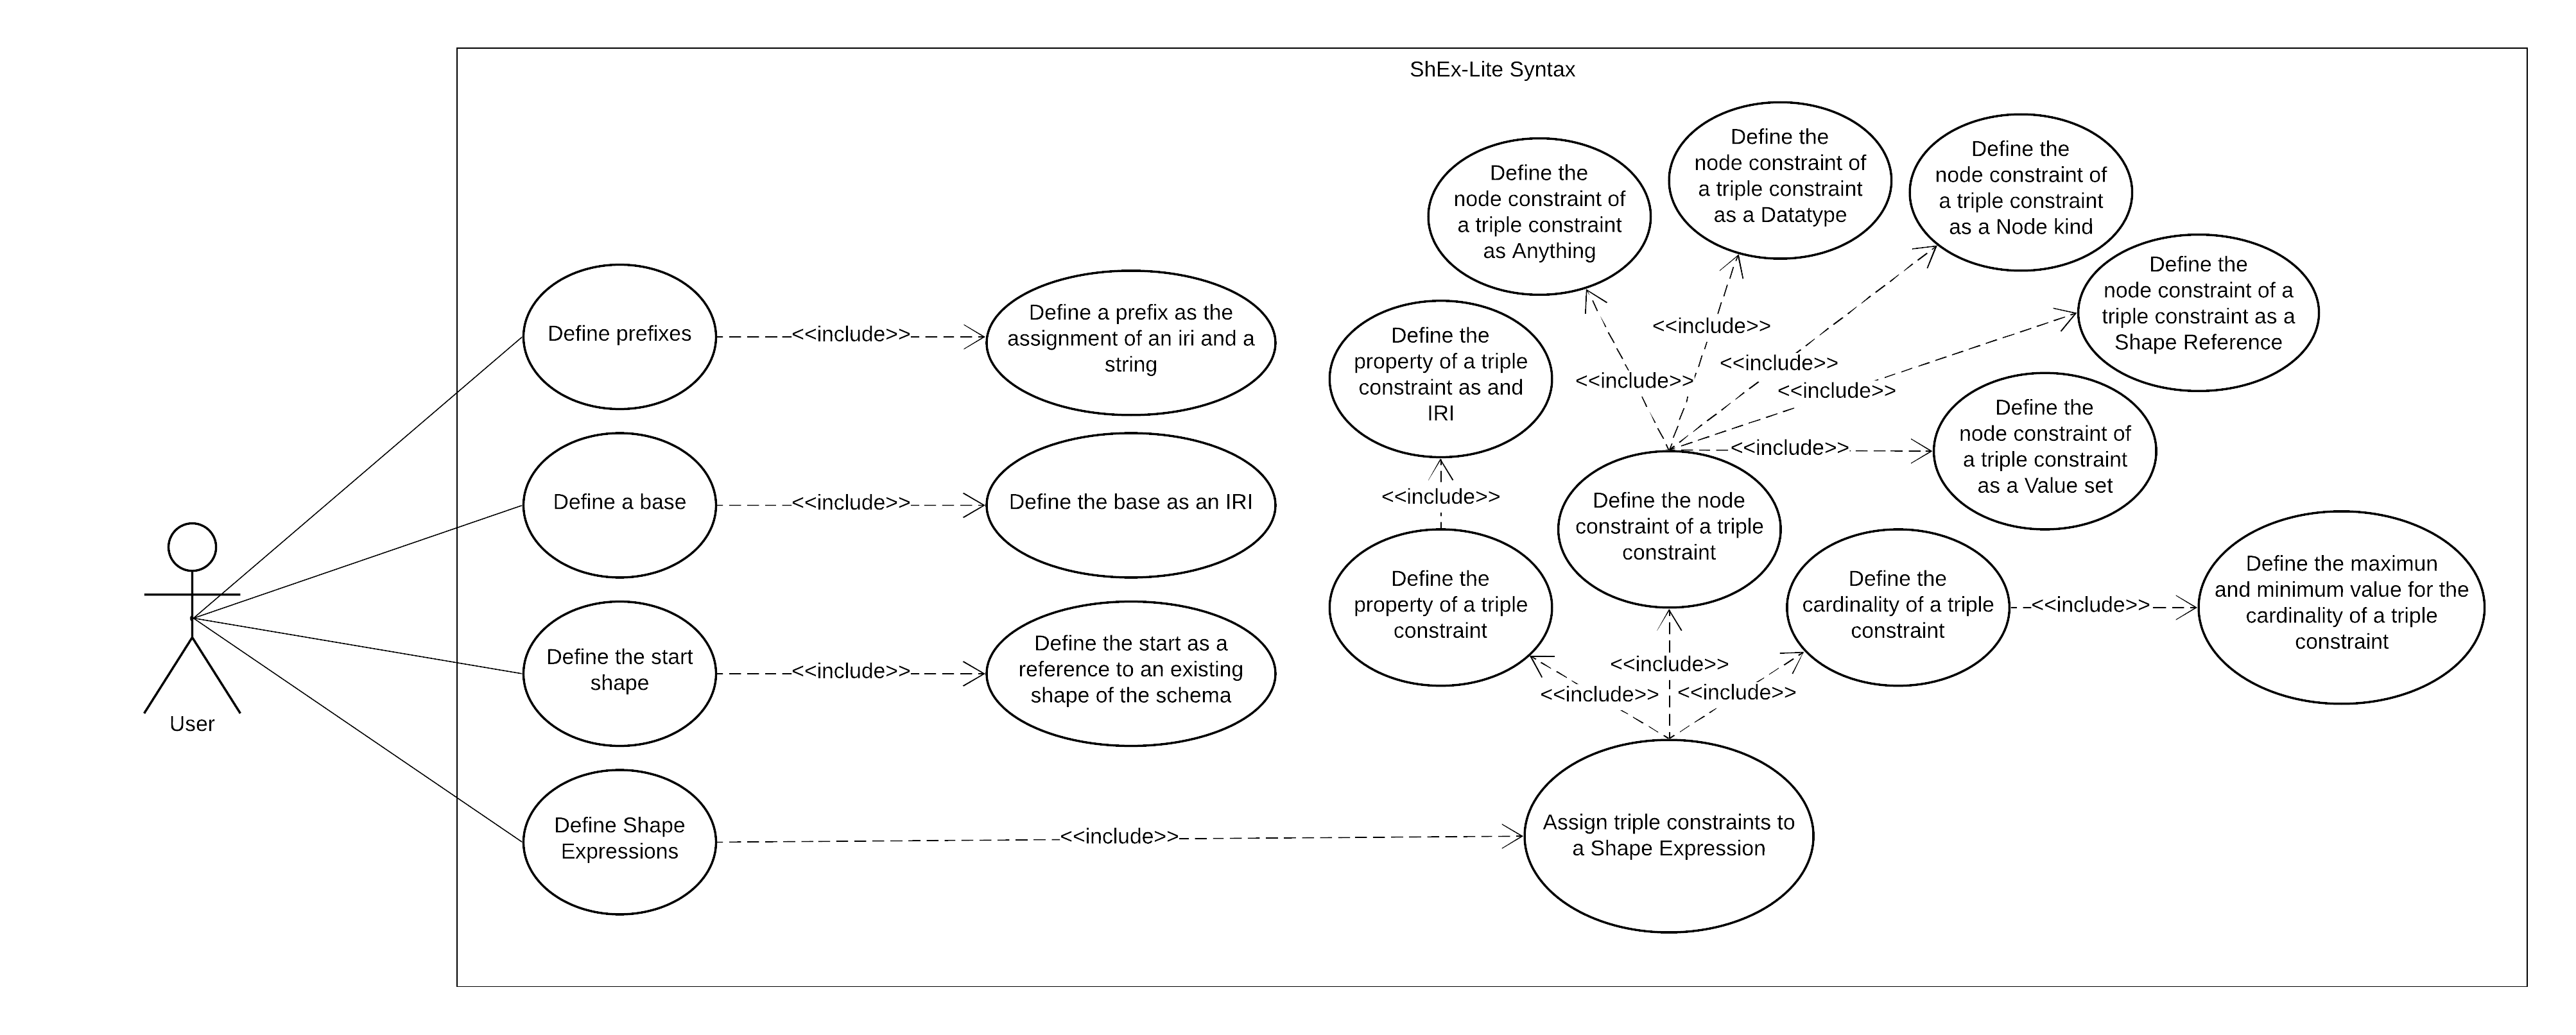
\includegraphics{shex-lite-syntax-use-case.png}
	\caption[ShEx-Lite syntax use case]{ShEx-Lite syntax use case.}
	\labfig{shex-lite-syntax-use-case}
\end{figure*}

Also the language will conservate most of the components of the shape expressions definitions from \texttt{ShEx}.
In our case a shape definition will be formed by a set of triple constraints. Each one of them will be of type
$Property$ $Constraint$ $Cardinality$.

\subsection{Syntax Requirements}
After we explore aims and the use cases that we expect for our syntax we can capture the requirements that grow
from them. It is important to remark that we are capturing the requirements of a syntax, not a system, therefore
we will only include the Syntax Requirements and the Quality Attributes that it must fullfil.

\subsubsection{Syntax Requirements}
The syntax requirements are those requirements that capture the functionality of the syntax, they will define
the actions that the syntax must allow to express.

\begin{enumerate}
    \item The syntax will allow to define prefixes.
    \begin{enumerate}
        \item A prefix definition will follow the ShEx specification.
    \end{enumerate}
    \item The syntax will allow to define a base.
    \begin{enumerate}
        \item A base definition will follow the ShEx specification.
    \end{enumerate}
    \item The syntax will allow to define the start shape expression.
    \begin{enumerate}
        \item The start shape expression will follow the ShEx specification.
    \end{enumerate}
    \item The system will allow to define shape expressions.
    \begin{enumerate}
        \item A shape expression will be formed by a shape label and a non-empty set of triple constraints.
        \begin{enumerate}
            \item A shape label will follow the ShEx specification.
            \item A triple constraint will be formed of the following elements:
            \begin{enumerate}
                \item The property. That will follow the ShEx specification.
                \item The node constraint. That will follow the ShEx specification.
                \item The cardinality. That will follow the ShEx specification.
            \end{enumerate}
        \end{enumerate}
    \end{enumerate}
\end{enumerate}

\subsubsection{Syntax Quality Attributes}
The syntax also includes some quality attributes that allow interoperability with other systems.
\begin{enumerate}
    \item The syntax will allow that any schema defined on it can be compiled by any other system that accepts ShEx Compact Syntax.
\end{enumerate}